\chapter{Infinite Odometry}

\section{Introduction}
In this work we present a novel algorithm for camera motion
estimation.  The novelty of the algorithm is in camera rotation
estimation procedure.  We rely on the fact that for scene points that
are infinitely far from the camera, the motion of the projected
(image) points may be described by an homography (the infinite
homography). For distant points this assumption is nearly true.  Our
algorithm starts by partitioning the scene points into two sets:
distant and near-by. Then, camera rotation is estimated from the
distant points and, subsequently, the translation is recovered from
the near-by points.

We present two versions of the algorithm: one for the monocular and
the other for the stereo settings.  These versions differ in the way
we partition points into the distant and the near-by ones and in the
way the algorithms estimate translation.

With respect to the classification of the visual odometry methods
given in the introduction, our work is local, feature based, stereo
odometry.  We do not use bundle adjustment, however the results of our
algorithm may be subsequently improved with some form of bundle
adjustment.

The outline of the our method:
\begin{enumerate}
\item Feature detection.  We use Harris~\cite{Harris1987} corners.
\item Feature matching. The matching is done both across the stereo
  pair images as well as previous vs.\ current pair.  We enforce
  epipolar constraint, chierality and use circle heuristics similar
  to~\cite{Geiger2011} to reject outliers.
\item Partition the scene points into two sets: distant and near-by.
\item Estimate the rotation of the camera from the distant points.
\item Estimate the translation of the camera from the near-by points.
\end{enumerate}

We choose the work~\cite{Geiger2011} as our baseline (our
implementation of their work).  The results in the
Section~\ref{sec:results} show that on the KITTI dataset our rotation
estimation method outperforms the baseline.

\section{Preliminaries and Notation}

\subsection{Image Point Mapping Related to Camera Motion}

Suppose the camera matrices are those of a calibrated stereo rig
$\mathrm{P}$ and $\mathrm{P}'$ with the world origin at the first
camera

\begin{equation}
\mathrm{P = K[I\ |\ 0],\quad P'=K'[R\ |\ \mathbf{t}]}.
\end{equation}

Consider the projections of a 3D point $\mathbf{X}=(X,Y,Z,1)^T$ into the image
planes of both views:

\begin{equation}
\mathrm{\mathbf{x} = P\mathbf{X}, \quad \mathbf{x}' = P'\mathbf{X}}.
\end{equation}

If the image point is normalized as $\mathbf{x} = (x,y,1)^T$ then
\[
\mathbf{x}Z = \mathrm{P\mathbf{X} = K[I\ |\ 0]\mathbf{X} = K}(X,Y,Z)^T.
\]

It follows that $(X,Y,Z)^T = \mathrm{K^{-1}}\mathbf{x}Z$, and:
\begin{align}
  \mathbf{x}' &= \mathrm{K'[R\ |\ \mathbf{t}]}(X,Y,Z,1)^T \\
  &= \mathrm{K'R}(X,Y,Z)^T + \mathrm{K'\mathbf{t}}\\
  &= \mathrm{K'RK^{-1}}\mathbf{x}Z + \mathrm{K'\mathbf{t}}.
\end{align}

We divide both sides by $Z$ to obtain the mapping of an image point $\mathbf{x}$ to image point $\mathbf{x}'$

\begin{equation}
  \label{eq:general_point_motion}
  \mathbf{x}' = \mathrm{K'RK^{-1}}\mathbf{x} + \mathrm{K'}\mathbf{t}/Z = \mathrm{H_\infty}\mathbf{x}+ \mathrm{K'}\mathbf{t}/Z = \mathrm{H_\infty}\mathbf{x} + \mathbf{e'}/Z.
\end{equation}

$\mathrm{H_\infty}$ is the infinite homography that transfers the
points at infinity to the points at infinity.  If $\mathrm{R = I}$
(e.g., pure translation) the point $\mathbf{x}$ will undergo a motion
along a corresponding epipolar line:
\begin{equation}
\mathbf{x}' = \mathbf{x}+ \mathrm{K'}\mathbf{t}/Z = \mathbf{x}+\mathbf{e}'/Z.
\end{equation}

If $\mathbf{t} = \mathbf{0}$ the motion of the point may be represented by a homography:
\begin{equation}
\mathbf{x}' = \mathrm{H_\infty}\mathbf{x}.
\end{equation}

\begin{figure}[h]
  \centering
  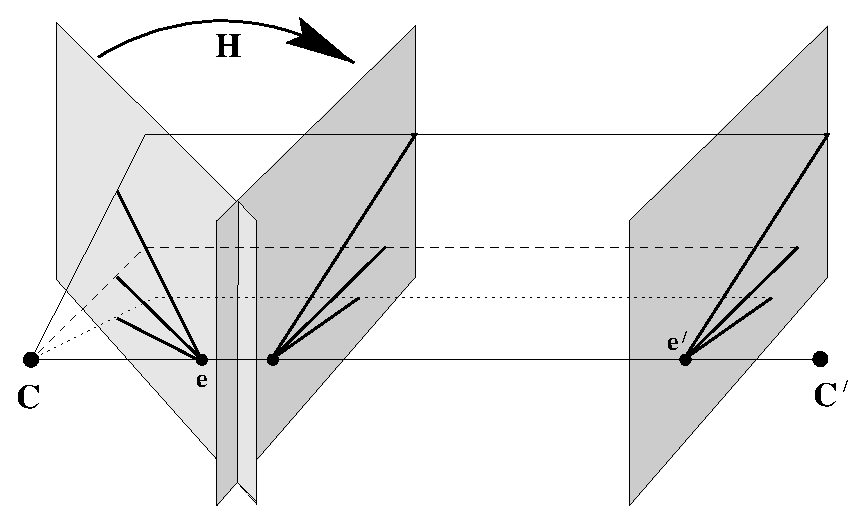
\includegraphics[scale=.5]{fig89}
  \caption{(Adapted from~\cite{Hartley2004}) The effect of the camera motion on
    the image points may be viewed as a two-step process: mapping by a
    homography $\mathrm{H_\infty}$ followed by a motion along the corresponding
    epipolar lines.}
  \label{fig:two_step_motion}
\end{figure}

In a general case the mapping of an image point $\mathbf{x}$ into
$\mathbf{x}'$ may be viewed as a two step process: transformation by a
homography which simulates a pure rotational motion of the camera
followed by an offset along the epipolar line which simulates a pure
translational motion of the camera, see
Figure~\ref{fig:two_step_motion}.

\section{Motion Estimation}\label{sec:moest}

Our strategy to attack the problem is to separate it into two smaller
sub-problems: rotation estimation and translation estimation. The
algorithm relies on the ability to partition the scene points into two
sets: the distant and the near-by ones.  The distant points are used
for rotation estimation while the near-by ones take part in the
translation estimation.

First, the stereo algorithm is presented, followed by the monocular
one.  The main difference is in the translation estimation part. While
it is possible to implement a stereo-like algorithm in the monocular
setting as well, it suffers from the scale drift.  Thus, we propose a
different technique.


\subsection{Stereo}\label{sec:stereo_moest}
\paragraph{Partitioning the points} To partition the points in the
stereo case we hard-threshold their $Z$-coordinates (the threshold is
a parameter of the algorithm).  The depth of the points was computed
by stereo triangulation.

\paragraph{Rotation Estimation:}\label{sec:rotation_estimation}
We use distant points to estimate rotation $\mathrm{R}$ (i.e., near-by
points do not take part in rotation estimation). As Eq.
(\ref{eq:general_point_motion}) states:

\begin{equation}
  \mathbf{x}' = \mathrm{KRK^{-1}}\mathbf{x} + \mathrm{K}\mathbf{t}/Z.
\end{equation}

The total motion of the feature point in the image plane may be viewed
as a two-step process (the order is not important): transformation by
homography $\mathrm{H_\infty} = \mathrm{KRK^{-1}}$ followed by
displacement along the line defined by the epipole $e'$ and the point
$\mathrm{H_\infty}\mathbf{x}$.  The magnitude of the displacement
along the epipolar line depends on the camera translation and the
inverse depth of the point, see Figure~\ref{fig:feature_motion}.

\begin{figure}[h]
  \centering
  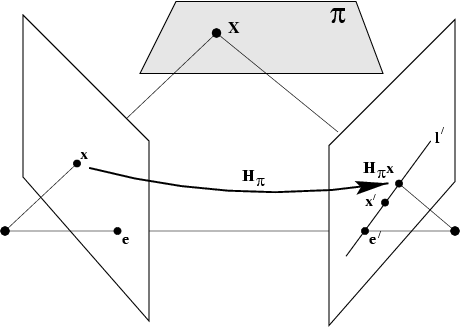
\includegraphics[scale=.5]{fig85_adapted}
  \caption{(Adapted from~\cite{Hartley2004}) The homography $H_\pi$ transfers the point onto a corresponding epipolar line.  The displacement along the epipolar line depends on the inverse depth of the point and the camera translation magnitude.}
  \label{fig:feature_motion}
\end{figure}                                                             %

Our estimation algorithm consists of initialization and non-linear
refinement.
\paragraph{Initialization:} to compute the initial estimate of the rotation
parameters we assume that for the distant points (s.t., $\norm{\mathbf{t}}/Z \ll \norm{\mathrm{H_\infty}\mathbf{x}}$):

\begin{equation}\label{eq:homography_transfer}
  \mathbf{x}' \approx \mathrm{KRK^{-1}}\mathbf{x}.
\end{equation}

This assumption is justified by the fact that for the distant points
the displacement along the epipolar line is small. We multiply
both sides of Eq. (\ref{eq:homography_transfer}) by $\mathrm{K^{-1}}$
and denote $\mathbf{u'} = \mathrm{K^{-1}}\mathbf{x}$ and
$\mathbf{u} = \mathrm{K^{-1}}\mathbf{x}$:

\begin{equation}
  \mathbf{u'} = \mathrm{K^{-1}}\mathbf{x}' \approx \mathrm{RK^{-1}}\mathbf{x} = \mathrm{R}\mathbf{u}.
\end{equation}

Since $\mathbf{u}$ and $\mathbf{u}'$ are projective quantities, only
their directions are of importance, we normalize them to unit length
and denote normalized quantities by $\mathbf{\tilde{u}}$ and
$\mathbf{\tilde{u}}'$ respectively. We choose a sample of $n$ points
($n=3$) and stack them as columns of matrices $\mathrm{\tilde{U}}$ and
$\mathrm{\tilde{U}'}$ respectively.  We search for $\mathrm{R}$ that
solves the following minimization problem:

\begin{equation}\label{eq:absolute_orientation}
\underset{\mathrm{R}}{\text{argmin}}\ \norm{\mathrm{\tilde{U}'-R\tilde{U}}}_2.
\end{equation}

Eq. (\ref{eq:absolute_orientation}) is known as the absolute
orientation problem (see e.g.,~\cite{Horn1987}) and its solution
provides an initial estimate for the subsequent non-linear
optimization problem.

\paragraph{Refinement:} The idea of the refinement is this: the
residual vector $\mathrm{H}_\infty\mathbf{x} - \mathbf{x}'$ may be
viewed as a sum of a vector orthogonal to the epipolar line and the
vector parallel to it.  We search for the camera rotation that ignores
the parallel component (we view it as a ``legal'' bias) while trying
to minimize the orthogonal one.  We define the point residual as the
orthogonal distance to the corresponding epipolar line and minimize
the sum of squared residuals for all points.  We do so, because, as
Eq. (\ref{eq:general_point_motion}) suggests, after we compensate for
a rotation, the point is still allowed to move along the epipolar
line.

Consider the objective:

\begin{equation}\label{eq:refinement_objective}
  \begin{split}
    \mathrm{R(v,\theta)} = \underset{v,\ \theta}{\mathrm{argmin}}
    \sum_{i=1}^N{r_i}^2\quad \text{s.t.}\quad r_i&=n_i\cdot (\mathbf{x}_i'-H_\infty(v,\theta)\mathbf{x}_i) \\
    \text{where}\ n_i &= (\mathrm{F}\mathbf{x}_i)_\perp
  \end{split}
\end{equation}
$\mathrm{H_\infty}(v,\theta) = \mathrm{KR(v,\theta)K^{-1}}$ is the
homography that transforms the image points in Eq.
(\ref{eq:general_point_motion}). It depends on a known camera
intrinsic matrices $\mathrm{K}$ and a rotation matrix $\mathrm{R}$.
We choose to parameterize the rotation by an angle $\theta$ and an
axis $v$.  $\mathrm{F}$ denotes the fundamental matrix that
corresponds to two subsequent stereo rig poses and is computed
elsewhere. $\mathrm{F}\mathbf{x}_i$ denotes the epipolar line that
corresponds to $\mathbf{x}_i$ in the second image and
$(\mathrm{F}\mathbf{x}_i)_\perp$ is the normal to this line.
We solve the minimization problem
(\ref{eq:refinement_objective}) by means of the Levenberg-Marquardt
optimization algorithm.

To make the estimation robust we wrap the initialization procedure
into the RANSAC iterations.  We choose the strongest consensus
estimate and its support set as an input for the solution of the
Eq. (\ref{eq:refinement_objective}).

\paragraph{Translation Estimation (1-point
  algorithm)}\label{sec:stereo_trans} To estimate
the translation we use only the near-by points.  First, we triangulate
these points in the previous stereo pair to obtain their 3-D
locations, and then iteratively minimize the sum of reprojection
errors into the current frame.

The reprojection of point $\mathbf{X}=(X,Y,Z,1)^T$ into the current
left image is given by:
\begin{equation}
  \pi^{(l)}(\mathbf{X};\mathbf{t}) =  K\Bigl[ \mathrm{R}\ |\ \mathbf{t} \Bigr]\mathbf{X}.
\end{equation}
and the reprojection of the same point into the current right image
($b$ is the baseline of the stereo-rig) is given by:
\begin{equation}
  \pi^{(r)}(\mathbf{X};\mathbf{t}) =  K\Bigl[ \mathrm{R}\ |\ \mathbf{t} \Bigr](\mathbf{X} - (b,0,0,0)^T),
\end{equation}

We use the Levenberg-Marquardt algorithm to iteratively minimize the
sum of squared reprojection errors (starting from
$\mathbf{t}=\mathbf{0}$):
\begin{equation}
\norm{\mathbf{x'} - \pi^{(l)}(\mathbf{X};\mathbf{t})}^2 + \norm{\mathbf{x'} - \pi^{(r)}(\mathbf{X};\mathbf{t})}^2.
\end{equation}

There are three unknown parameters, since
$\mathbf{t} = (t_x,t_y,t_z)^T$, thus a single 3-D point provides
enough constraints to determine $\mathbf{t}$.

\subsection{Mono}\label{sec:mono_moest}

The stereo setup has an advantage over the monocular one in the sense
that it provides the algorithm with more information (e.g., the
calibration and the additional image at each camera position).  These
advantages come at a price, e.g., the cameras need to be synchronized
and the computational resource requirements climb.  These make
monocular setups and the related algorithms more attractive.  In the
following section we present the version of our algorithm, adapted for
the monocular setup.

Given two sets of matching image points $\mathbf{x}_i, \mathbf{x}_i'$
from two subsequent frames $I_1, I_2$ respectively, we estimate the
camera motion between these frames. Similar to the stereo algorithm in
Section \ref{sec:stereo_moest} the algorithm first partitions the
points and then estimates the rotation followed by the estimation of
the translation direction (it is well known that the magnitude of the
camera translation is unavailable in the monocular setting).

\paragraph{Partitioning the points} \label{sec:mono_split} To estimate
the rotation of the camera as in the Eq. (\ref{sec:moest}), it is
required to partition the set of the image points into the distant
ones and the near-by ones.  While in the stereo setting we may
triangulate the points and threshold their depths, in the monocular
setting this can not be done.  This section proposes a method to
perform the aforementioned partition in the monocular setting.

Consider the subsequent images $I_1, I_2, I_3$ taken by a moving
camera at the locations $O_1,O_2$ and $O_3$ respectively. We assume
the image points $\mathbf{x}_i$ in $I_1$ are known to be distant
relative to the camera at $O_1$.  The magnitude of the camera
translation is small relative to the distant points depths, thus we
assume that these points are distant w.r.t.\ the camera at $O_2$ and
$O_3$ as well.  Some of these points will be lost in $I_3$, thus it is
desirable to known which of the points tracked from $I_2$ to $I_3$
(which are not part of $\mathbf{x}_i$'s) are distant (denote these by
$\mathbf{y}_j$).

The real baselines $t_1=\norm{O_1-O_2}$ and $t_2=\norm{O_2-O_3}$ are
unknown and thus we can not use them to obtain real depths of the
points.

We use the following procedure to classify the newly tracked points in
$I_2$ as distant:
\begin{enumerate}
\item Set $t_1=1$ and triangulate the distant points $\mathbf{x}_i$ to
  obtain the depths $Z_i$
\item Set $t_2=1$ and triangulate the points $\mathbf{y}_j$ to obtain
  the depths $Z_j$
\item Classify the point $y_j$ to be distant if
  $Z_j>\underset{i}{\text{min}}\ Z_i$.
\end{enumerate}

While the assumption $t_1 \approx t_2$ is acceptable for the KITTI
dataset, it may be improved on by computing the $t_1/t_2$ ratio (by
minimizing the reprojection errors of $\mathbf{x}_i$ into $I_3$,
similar to the translation estimation described in the Section
\ref{sec:stereo_trans}).

To initialize the monocular algorithm we may further assume that the
initial motion is a pure translation and thus the points with small
disparity are the distant ones (disparity being the magnitude of the
motion in the image plane).

\paragraph{Rotation Estimation} is exactly as in the Section 
\ref{sec:rotation_estimation}. Denote the estimated rotation by
$\mathrm{R}$ and the corresponding homography by $\mathrm{H}$.

\paragraph{Translation Estimation} is as follows. Compensate the
rotation by computing $\mathbf{y}_i = \mathrm{H_\infty}\mathbf{x}_i$.  We optimize over the location of
the epipole $e$ and minimize the orthogonal distances of the points to
their corresponding epipolar lines:

\begin{align}
  \underset{e}{\text{argmin}}\ \sum_i{d(l_i,\mathbf{y}_i)+d(l_i,\mathbf{x}_i')}\ \text{s.t.}\  d(e,l_i) & =0\ \text{while}\ l_i = \underset{l}{\text{argmin}}\ d(l,\mathbf{x}_i') + d(l,\mathbf{y}_i)
\end{align}

We define the epipolar line $l_i$ to be the line that passes through
the epipole and its distance to $\mathbf{x}_i'$ and $\mathbf{y}_i$ is
minimal. $d(l,\mathbf{x})$ denotes the distance from the line $l$ to
the point $\mathbf{x}$.  The epipole provides us with the translation
direction of the camera.

\section{Experimental Results}\label{sec:results}

\subsection{The Choice of Features}
We chose to evaluate our algorithm on the KITTI
dataset~\cite{Geiger2012}, which is a de-facto standard for the
visual odometry research works.

\paragraph{Feature Detector/Descriptor:} We use Harris
~\cite{Harris1988} corner detector. It is fast, well localized and
(most important) Harris corners are abundant in urban scenes we work
with. We detect corners in each new image and then match them to
obtain putative matches.  We tune sensitivity threshold of the
detector in such a way, that we are left with about five hundred
putative matches after matching and pruning.  We extract a square
patch of $7\times 7$ pixels centered at the corner point and use this
vector as feature descriptor.

We would like to point out that our method may be used with any
feature detector that would allow to match features across images. The
choice of feature detector should be viewed as a parameter to the
algorithm and mainly depends on the images at test.

\paragraph{Feature Matching:} We use sum-of-square differences (SSD)
of feature descriptors as a metric function when matching
features. For each feature we choose a single best match w.r.t. the
metric function in the other image. We employ a number of heuristics
to prune outliers:
\begin{itemize}
\item Reciprocity: features $a$ and $b$ match only if $a$ matches $b$
  and $b$ matches $a$
\item Epipolar constraint: we work with calibrated stereo pair.  When
  we match features across images of stereo pair, the search is
  one-dimensional, i.e., along the horizontal epipolar line.  This
  heuristic is not used when matching features across subsequent
  frames.
\item Chierality (visibility): also used when matching features across
  stereo pair images.  We triangulate the features to obtain the 3-D
  point and keep the match only if the 3-D point is visible in both
  cameras.
\item Circular match: similar to ~\cite{Geiger2011} we keep only those
  matches that form a circle.
\end{itemize}

\subsection{Experimental Results}

The Tables \ref{table:rot_err} and \ref{table:trans_err} present the
results of the experiments for the KITTI dataset. The columns denote
the number of the sequence.  The rows denote the algorithm: SS is the
baseline, HX is the stereo version of the algorithm, HG is the
monocular version.  The numbers are the mean error for the
corresponding sequence with the last column is the mean error for the
dataset. The error computation method is described
in~\cite{Geiger2012}.

\paragraph{Stereo} In this set of experiments we ran our algorithm in
its stereo mode as described in the Section \ref{sec:stereo_moest}.
Table \ref{table:rot_err} and \ref{table:trans_err} present the
rotation and the translation errors respectively in the row HX. The
columns marked bold are those that our algorithm outperforms the
baseline (on 9 of 11 sequences). The results show that our algorithm improves the
rotation results over the benchmark algorithm and successfully
competes with it in the translation estimation.

\paragraph{Mono} In an additional set of experiments we ran our
algorithm in a monocular mode. Monocular motion estimation lacks a
scale parameter. In order to compare the results we set the
scale of the translation to be that of the stereo algorithm.  Feature
point selection/partition was done without using any stereo
information and the motion estimation was done as explained in the
Section~\ref{sec:mono_moest}.

\section{Conclusions and Discussion}
This work presents a novel visual odometry algorithm.  The novelty of
the algorithm is in its rotation estimation method.  The rotation is
estimated by means of the infinite homography.  The algorithm may be
used both in the stereo and in the monocular setting.

The strengths of the presented algorithm are in its ability to split
the motion estimation problem into two smaller problems and to operate
directly on the image points instead of on the computed 3-D
quantities.  Splitting the problem helps because each sub-problem is
easier to solve.  The ability to partition the points into the distant
and the near-by ones is what allows us to separate the rotation and
the translation estimation.  

The stereo version of the algorithm shows better performance, but the
monocular version has the advantage of being a more practical one.
Indeed the authors in~\cite{Geiger2012} report that they re-calibrate
the cameras before each drive, which is hardly possible in real world
installations.

\begin{table}
  \centering
  \caption{Rotation errors for the KITTI sequences [deg/m]}
  \label{table:rot_err}
  \smallskip\noindent
  \resizebox{\linewidth}{!}{%
    \begin{tabular}{|c|c|c|c|c|c|c|c|c|c|c|c|c|}
\hline
 & 00 & 01 & 02 & 03 & 04 & 05 & 06 & 07 & 08 & 09 & 10 & mean \\
\hline
SS & 3.95e-04 & 1.98e-04 & 4.11e-04 & 1.07e-03 & 8.03e-04 & 3.49e-04 & 4.72e-04 & 2.96e-04 & 3.69e-04 & 3.44e-04 & 4.82e-04 & 4.71e-04 \\
\hline
HX & \textbf{2.70e-04} & \textbf{1.75e-04} & \textbf{4.10e-04} & \textbf{6.51e-04} & \textbf{6.04e-04} & 3.95e-04 & \textbf{3.77e-04} & \textbf{2.37e-04} & \textbf{3.23e-04} & \textbf{3.22e-04} & 5.66e-04 & \textbf{3.93e-04} \\
\hline
HG & 8.72e-04 & 3.89e-04 & 6.28e-04 & 1.07e-03 & 5.99e-04 & 6.96e-04 & 3.31e-04 & 8.12e-04 & 8.13e-04 & 6.82e-04 & 5.23e-04 & 6.74e-04 \\

\hline
\end{tabular}

  }
\end{table}

\begin{table}
  \centering
  \caption{Translation errors for the KITTI sequences \% }
  \label{table:trans_err}
  \smallskip\noindent
  \resizebox{\linewidth}{!}{%
    \centering
\begin{tabular}{|c|c|c|c|c|c|c|c|c|c|c|c|c|}
\hline
 & 00 & 01 & 02 & 03 & 04 & 05 & 06 & 07 & 08 & 09 & 10 & mean \\
\hline
SS & 4.40e+00 & 9.25e+00 & 4.03e+00 & 1.22e+01 & 5.06e+00 & 2.80e+00 & 4.37e+00 & 2.21e+00 & 4.12e+00 & 5.25e+00 & 5.60e+00 & 5.39e+00 \\
\hline
HX & 3.07e+00 & 1.08e+01 & 3.80e+00 & 7.94e+00 & 3.82e+00 & 4.06e+00 & 3.99e+00 & 1.67e+00 & 3.28e+00 & 3.77e+00 & 5.65e+00 & 4.72e+00 \\
\hline
HG & 1.21e+01 & 1.48e+01 & 8.72e+00 & 1.33e+01 & 8.62e+00 & 8.37e+00 & 4.46e+00 & 7.93e+00 & 9.76e+00 & 1.16e+01 & 8.36e+00 & 9.82e+00 \\
\hline
\end{tabular}

  }
\end{table}
